\documentclass[12pt, spanish]{article}
\usepackage[spanish]{babel}
\selectlanguage{spanish}
\usepackage{natbib}
\usepackage{url}
\usepackage[utf8x]{inputenc}
\usepackage{graphicx}
\graphicspath{{images/}}
\usepackage{parskip}
\usepackage{fancyhdr}
\usepackage{vmargin}
\usepackage{multirow}
\usepackage{float}
\usepackage{chngpage}

\usepackage{subcaption}

\usepackage{hyperref}
\usepackage[
    type={CC},
    modifier={by-nc-sa},
    version={4.0},
]{doclicense}

\hypersetup{
    colorlinks=true,
    linkcolor=blue,
    filecolor=magenta,      
    urlcolor=cyan,
}

% para codigo
\usepackage{listings}
\usepackage{xcolor}



%% configuración de listings

\definecolor{listing-background}{HTML}{F7F7F7}
\definecolor{listing-rule}{HTML}{B3B2B3}
\definecolor{listing-numbers}{HTML}{B3B2B3}
\definecolor{listing-text-color}{HTML}{000000}
\definecolor{listing-keyword}{HTML}{435489}
\definecolor{listing-identifier}{HTML}{435489}
\definecolor{listing-string}{HTML}{00999A}
\definecolor{listing-comment}{HTML}{8E8E8E}
\definecolor{listing-javadoc-comment}{HTML}{006CA9}

\lstdefinestyle{eisvogel_listing_style}{
  language         = c++,
%$if(listings-disable-line-numbers)$
%  xleftmargin      = 0.6em,
%  framexleftmargin = 0.4em,
%$else$
  numbers          = left,
  xleftmargin      = 0em,
 framexleftmargin = 0em,
%$endif$
  backgroundcolor  = \color{listing-background},
  basicstyle       = \color{listing-text-color}\small\ttfamily{}\linespread{1.15}, % print whole listing small
  breaklines       = true,
  frame            = single,
  framesep         = 0.19em,
  rulecolor        = \color{listing-rule},
  frameround       = ffff,
  tabsize          = 4,
  numberstyle      = \color{listing-numbers},
  aboveskip        = 1.0em,
  belowskip        = 0.1em,
  abovecaptionskip = 0em,
  belowcaptionskip = 1.0em,
  keywordstyle     = \color{listing-keyword}\bfseries,
  classoffset      = 0,
  sensitive        = true,
  identifierstyle  = \color{listing-identifier},
  commentstyle     = \color{listing-comment},
  morecomment      = [s][\color{listing-javadoc-comment}]{/**}{*/},
  stringstyle      = \color{listing-string},
  showstringspaces = false,
  escapeinside     = {/*@}{@*/}, % Allow LaTeX inside these special comments
  literate         =
  {á}{{\'a}}1 {é}{{\'e}}1 {í}{{\'i}}1 {ó}{{\'o}}1 {ú}{{\'u}}1
  {Á}{{\'A}}1 {É}{{\'E}}1 {Í}{{\'I}}1 {Ó}{{\'O}}1 {Ú}{{\'U}}1
  {à}{{\`a}}1 {è}{{\'e}}1 {ì}{{\`i}}1 {ò}{{\`o}}1 {ù}{{\`u}}1
  {À}{{\`A}}1 {È}{{\'E}}1 {Ì}{{\`I}}1 {Ò}{{\`O}}1 {Ù}{{\`U}}1
  {ä}{{\"a}}1 {ë}{{\"e}}1 {ï}{{\"i}}1 {ö}{{\"o}}1 {ü}{{\"u}}1
  {Ä}{{\"A}}1 {Ë}{{\"E}}1 {Ï}{{\"I}}1 {Ö}{{\"O}}1 {Ü}{{\"U}}1
  {â}{{\^a}}1 {ê}{{\^e}}1 {î}{{\^i}}1 {ô}{{\^o}}1 {û}{{\^u}}1
  {Â}{{\^A}}1 {Ê}{{\^E}}1 {Î}{{\^I}}1 {Ô}{{\^O}}1 {Û}{{\^U}}1
  {œ}{{\oe}}1 {Œ}{{\OE}}1 {æ}{{\ae}}1 {Æ}{{\AE}}1 {ß}{{\ss}}1
  {ç}{{\c c}}1 {Ç}{{\c C}}1 {ø}{{\o}}1 {å}{{\r a}}1 {Å}{{\r A}}1
  {€}{{\EUR}}1 {£}{{\pounds}}1 {«}{{\guillemotleft}}1
  {»}{{\guillemotright}}1 {ñ}{{\~n}}1 {Ñ}{{\~N}}1 {¿}{{?`}}1
  {…}{{\ldots}}1 {≥}{{>=}}1 {≤}{{<=}}1 {„}{{\glqq}}1 {“}{{\grqq}}1
  {”}{{''}}1
}
\lstset{style=eisvogel_listing_style}


\usepackage[default]{sourcesanspro}

\setmarginsrb{2 cm}{1 cm}{2 cm}{2 cm}{1 cm}{1.5 cm}{1 cm}{1.5 cm}

\title{Práctica 1:\\
PAR - Greedy y Busqueda Local  \hspace{0.05cm} }                           
\author{Antonio David Villegas Yeguas}                             
\date{\today}                                           

\renewcommand*\contentsname{hola}

\makeatletter
\let\thetitle\@title
\let\theauthor\@author
\let\thedate\@date
\makeatother

\pagestyle{fancy}
\fancyhf{}
\rhead{\theauthor}
\lhead{\thetitle}
\cfoot{\thepage}

\begin{document}

%%%%%%%%%%%%%%%%%%%%%%%%%%%%%%%%%%%%%%%%%%%%%%%%%%%%%%%%%%%%%%%%%%%%%%%%%%%%%%%%%%%%%%%%%

\begin{titlepage}
    \centering
    \vspace*{0.3 cm}
    
\includegraphics[scale = 0.50]{ugr.png}\\[0.7 cm]
    %\textsc{\LARGE Universidad de Granada}\\[2.0 cm]   
    \textsc{\large 3º CSI 2019/20 - Grupo 1}\\[0.5 cm]            
    \textsc{\large Grado en Ingeniería Informática}\\[0.5 cm]              
    \rule{\linewidth}{0.2 mm} \\[0.2 cm]
    { \huge \bfseries \thetitle}\\
    \rule{\linewidth}{0.2 mm} \\[1 cm]
    
    \begin{minipage}{0.4\textwidth}
        \begin{flushleft} \large
            \emph{Autor:}\\
            \theauthor\\ 
			 \emph{DNI:}\\
            77021623-M
            \end{flushleft}
            \end{minipage}~
            \begin{minipage}{0.4\textwidth}
            \begin{flushright} \large
            \emph{Asignatura: \\
            Metaheurísticas}   \\     
            \emph{Correo:}\\
            advy99@correo.ugr.es           
        \end{flushright}
    \end{minipage}\\[0.5cm]
  
    {\large \thedate}\\[0.5cm]
    {\url{https://github.com/advy99/MH/}}
    {\doclicenseThis}
 	
    \vfill
    
\end{titlepage}

%%%%%%%%%%%%%%%%%%%%%%%%%%%%%%%%%%%%%%%%%%%%%%%%%%%%%%%%%%%%%%%%%%%%%%%%%%%%%%%%%%%%%%%%%

\tableofcontents
\pagebreak

%%%%%%%%%%%%%%%%%%%%%%%%%%%%%%%%%%%%%%%%%%%%%%%%%%%%%%%%%%%%%%%%%%%%%%%%%%%%%%%%%%%%%%%%%


\section{Descripción del problema de la asignación con restricciones.}

El problema de la asignación con restricciones consiste en una generalización del problema de agrupamiento clásico, bastante común en \textit{Machine Learning}.

El problema del agrupamiento clásico es un problema en el que se recibe como entrada las características de un conjunto de elementos y el número de agrupaciones a realizar, para resolver el problema tendremos como objetivo realizar dichas agrupaciones de los distintos elementos con el fin de organizarlos acorde a las características dadas. Llamaremos a estas agrupaciones \textit{Clusters}.

Como extensión a este problema, nosotros trabajaremos sobre el problema de asignación con restricciones (de ahora en adelante PAR). PAR se basa en el problema del agrupamiento clásico, pero añadiendo al problema restricciones entre los propios elementos, es decir, las distintas parejas que podemos formar con los datos tendrán asociadas restricciones de dos tipos:

\begin{itemize}
	\item{Must-Link (ML): Dados dos datos $D_1$ y $D_2$, si estos datos tienen asociada una restricción ML deberán tener asignado el mismo cluster.}
	\item{Cannot-Link (CL): Dados dos datos $D_1$ y $D_2$, si estos datos tienen asociada una restricción CL deberán tener asignado distinto cluster.}
\end{itemize}

Nosotros trataremos estas restricciones como restricciones débiles, es decir, permitiremos que se incumplan pero penalizándolas, por lo tanto, el objetivo para resolver el PAR es minimizar la distancia de los elementos que conforman los distintos clusters, así como asegurarnos que no se incumple ninguna restricción.

Otra restricción fuerte del problema es que todos los clusters tienen que tener al menos un elemento.

Para comprobar que la distancia entre los elementos de los distintos clusters es mínima, tendremos las siguientes características asociadas a un cluster:

\begin{itemize}
	\item{Centroide: Valor promedio de los datos que conforman el cluster. Con este elementos obtendremos la representación del elemento central del cluster.}
	\item{Distancia media intra-cluster: Con este elemento mediremos como de disperso está nuestro cluster, es decir, si los elementos de un cluster están cercanos entre si.}
\end{itemize}

Además también contaremos con distintas características del PAR:

\begin{itemize}
	\item{Desviación general: Será la media de las desviaciones intra-cluster de los distintos clusters que conforman el PAR. Uno de nuestros objetivos será que este valor sea mínimo.}
	\item{\textit{Infeasibility}: Esta característica nos permitirá conocer cuantas restricciones se están incumpliendo en una posible solución del PAR. Otro de nuestros objetivos será que este valor sea mínimo.}
\end{itemize}

\newpage

\section{Descripción de la implementación común y representación del problema para su resolución.}

Para el desarrollo e implementación del programa que resolverá el PAR he decidido usar C++ como lenguaje de programación.

Para la representación del problema he decidido construir dos clases en C++, la clase PAR y la clase Cluster.



\subsection{Clase PAR:}


Esta clase contará con los siguientes atributos:

\begin{itemize}
	\item {Matriz que almacenará valores reales, donde estarán las características de los datos.}
	\item {Vector de objetos tipo Cluster con el que representaremos las agrupaciones a conseguir.}
	\item {Diccionario con las restricciones entre los distintos datos.}
	\item {Desviación general del problema.}
	\item {Mayor distancia entre dos los distintos datos del problema.}
	\item {\textit{Infeasibility} del problema}
\end{itemize}


\subsection{Clase Cluster:}

Con esta clase representaremos los elementos y operaciones internas de un cluster. Tendrá los siguientes atributos:

\begin{itemize}
	\item {Set que almacenará enteros, representando que elementos conforman dicho cluster.}
	\item {Vector de reales que representará el centroide.}
	\item {Valor real que representará la distancia intra-cluster de los elementos que lo conforman.}
	\item {Una referencia a la clase PAR asociada, con la que obtendremos los datos necesarios sin necesidad de duplicarlos.}
\end{itemize}

Es importante mencionar que la declaración de la clase Cluster se realiza dentro de la clase PAR, ya que no tiene sentido crear un cluster sin tener un problema asociado.


\newpage

\subsection{Representación:}

\subsubsection{Datos:}

Con respecto a la representación del problema, los datos son almacenados en una matriz de datos tipo \texttt{double}, cada fila representará un dato, y las columnas representarán las características de dicho dato.

\subsubsection{Restricciones:}

Las restricciones serán almacenadas en un diccionario, donde la clave será la pareja de datos afectada por la restricción y el valor será 1 si la restricción es ML o -1 si es CL. He decidido usar esta representación ya que nos permite almacenar la información de forma eficiente sin tener que almacenar los elementos que no tiene restricciones entre sí, nos permite acceder a los elementos de una forma más rápida que con una lista (aunque no tanto comparado con una matriz, pero gracias al operador \texttt{find} de la clase esto apenas se nota) y podemos recorrer las restricciones secuencialmente de una forma rápida gracias a los iteradores disponibles en la clase diccionario de C++.


Con esta representación de los datos y las restricciones, las distintas operaciones antes comentadas se pueden resolver de forma sencilla generalizando el número de generalizando el número de características, independientemente del problema.


\subsubsection{Solución:}

Para representar la solución he decido, como he comentado anteriormente, que la solución esté compuesta por un vector de objetos tipo cluster, a pesar de que esta representación no será valida para futuras prácticas, es mucho más sencillo y práctico trabajar con ella en la primera práctica, ya que al separar los distintos clusters en su propio objeto podemos realizar las operaciones que afecten a los clusters de forma mucho más rápida y permitiendo la factorización del problema, ya que por ejemplo, seremos capaces de recalcular el centroide de un cluster sin tener que tener en cuenta los demás, o separar los elementos.

La representación dada en clase (vector de enteros de tamaño N siendo N el número de datos, y cada posición del vector se le asocia un número, que será el cluster al que pertenece) es de gran utilidad en la práctica 2, por lo que tenemos una función que nos intercambiará entre estas soluciones, es decir, una función que dado un vector de clusters nos devolverá un vector de enteros con las asignaciones del argumento dado.

\begin{lstlisting}
//vector de ints en el que devolveremos la solución
vector_sol 

Para todo cluster i en el vector de clusters:
	Para todo elemento j en el cluster i:
		vector_sol[j] = i;
		
Devolver vector_sol

\end{lstlisting}


\subsubsection{Operaciones sobre los clusters:}

Los clusters tendrán principalmente dos funciones que podremos realizar:

\begin{itemize}
	\item {Calcular el centroide}
	\item {Calcular la distancia media intra-cluster}
\end{itemize}

Para calcular el centroide basta con recorrer los elementos que conforman ese cluster (disponibles dentro de la clase Cluster) y calcular el punto medio.

\begin{lstlisting}
Para i = 0 hasta el tamaño del centroide (numero de caracteristicas de un dato) :
	centroide[i]=0.0d
	
Para cada elemento i del cluster:
	Para cada carasterictica j del elemento i:
		centroide[j] += problema.datos[i][j];
		
Para cada caracteristica i del centroide:
	centroide[i] /= num_elementos_cluster 
	
	
\end{lstlisting}

Para calcular la distancia media intra-cluster calcularemos el centroide y tras eso la distancia de todos los elementos al centroide.


\begin{lstlisting}
calcular_centroide();
distancia_intra_cluster = 0
	
Para cada elemento i del cluster:
	Para cada carasterictica j del elemento i:
		distancia_intra_cluster += problema.datos[i][j];
		
Para cada caracteristica i del centroide:
	distancia_intra_cluster /= num_elementos_cluster 
	
	
\end{lstlisting}

\newpage

\subsubsection{Operaciones sobre PAR:}

Sobre el problema podremos aplicar las siguientes operaciones:

\begin{itemize}
	\item {Calcular la desviación general.}
	\item {Buscar el cluster en el que se encuentra cierto elemento.}
	\item {Calcular \textit{Infeasibility} del estado actual del PAR.}
	\item {Calcular la distancia entre dos puntos del problema.}
\end{itemize}

Para calcular la desviación general haremos la media de las distintas desviaciones intra-cluster.


\begin{lstlisting}
desviacion_general = 0
	
Para cada elemento i del vector de clusters:
	clusters[i].calcular_desviacion_intra_cluster()
	desviacion_general += cluster[i].desviacion_intra_cluster()
		
desviacion_general /= clusters.size()	
	
\end{lstlisting}

Para buscar un elemento N dado por parámetro en los distintos clusters simplemente recorreremos el vector de clusters usando el operador find de la clase set, al estar ordenados y ser únicos, esto hará que esta operación sea muy rápida.

\begin{lstlisting}
encontrado = false
encontrado_en_cluster = -1

Mientras !encontrado Y para cada elemento i del vector clusters
	Si clusters[i].elementos.find(N) != clusters[i].elementos.end()
		encontrado = true	
		encontrado_en_cluster = i
		
return encontrado_en_cluster
	
\end{lstlisting}


Para calcular  \textit{Infeasibility} del PAR simplemente recorreremos el diccionario de restricciones, si encontramos dos elementos en distinto cluster y son ML sumamos 1 al total, y si encontramos dos elementos en el mismo cluster y tienen la restricción de CL sumamos 1 al total.

Solo comprobaremos si en el diccionario, la pareja de datos el primer elemento es mayor que el segundo. Esto lo hacemos para evitar contar dos veces la misma restricción, por ejemplo, si tenemos la restricción 0 con 1: ML, también tenemos la 1 con 0: ML, así que solo comprobaremos la 1 con 0. A pesar de usar el diccionario he decidido duplicar de esta forma las restricciones ya que a veces necesitaremos acceder sin tener en cuenta el orden de los datos.

\newpage

\begin{lstlisting}
infac = 0

Para cada elemento i de  restricciones
	Si i.first.first > i.first.second
		Si existe una restricción entre i.first.first e i.first.second
			c1 = buscar_elemento(i.first.first)
			c1 = buscar_elemento(i.first.second)
			
			Si c1 == c2 Y i.second == -1
				infac++
			Si c1 != c2 Y i.second == 1
				infac++
		
		
return infac
	
	
\end{lstlisting}




Tanto en PAR como en Cluster tendremos otras operaciones auxiliares relativas a los algoritmos de búsqueda o comparación, que explicaré más adelante.


\subsection{Calcular \textit{Infeasibility} parcial.}

Para hacer una factorización, además de poder calcular los atributos de los clusters de forma independiente sin necesidad de recalcular la de todos si no son modificados también necesitaremos una función que dado un cluster y un elemento nos calcula cuantas restricciones incumpliría si lo introducimos en dicho cluster.


\begin{lstlisting}
elemento: nos lo dan como argumento
cluster: nos lo dan como argumento

incumplidas = 0


Para todos los elementos i del cluster dado:
	Si i y elemento tienen una restricción Y dicha restricción == -1
		incumplidas++

Para los elementos j de los clusters != cluster:
	Si j y elemento tienen una restricción Y dicha restricción == 1
		incumplidas++



return incumplidas
	
	
\end{lstlisting}

\subsection{Función objetivo.}

En el caso del PAR nuestro objetivo será agrupar los datos en clusters incumpliendo el mínimo de restricciones.

Para cumplir la primera parte intentaremos que los datos estén lo menos dispersos con respecto a su centroide, por lo que intentaremos minimizar el total de las desviaciones intra-cluster, en resumen, \textbf{minimizar la desviación general}. 

Para la segunda parte, intentaremos minimizar el número de restricciones incumplidas penalizando las soluciones que más restricciones incumplan. Esta penalización se basará en sumar a la desviación general un valor entre 0 y la distancia más grande entre los datos del problema.

Esto lo conseguiremos con este factor, al que llamaremos $\lambda$:

$$ \lambda = \frac{D_{max}}{NumRestricciones} $$ 


De forma que si incumplimos todas las restricciones la solución la consideraremos mucho peor que otra con mayor desviación general pero menor restricciones incumplidas.

Nuestra función objetivo será:

$$ f = C + (\textit{Infeasibility} * \lambda) $$ 


\newpage

\section{Métodos de resolución del problema.}

\subsection{Algoritmo de Búsqueda Local.}

Este algoritmo se basa en partir de una solución inicial aleatoria, a partir de esa solución explorar una solución vecina, y si esta solución vecina es mejor que la actual, moverse a dicha solución.

Este algoritmo no nos asegurará obtener el optimo, solo nos garantiza obtener un mínimo local (puede que este mínimo local sea el optimo, pero no lo podemos asegurar).

El algoritmo solo cambiará una solución por otra mejor, por lo que el punto de inicio será muy importante.

Para desarrollar este algoritmo necesitamos varios componentes:
 
 \subsubsection{Generador de solución inicial aleatoria.}
 
 Primero he desarrollado una función que nos genera una solución aleatoria que cumple con las restricciones fuertes (todos los clusters tienen al menos un elemento).
 
 \begin{lstlisting}
vaciar_clusters()

indices_aleatorios = {0...datos.size()}

indices_aleatorios = random_shuffle(indices)

contador = 0

// nos aseguramos que cada cluster tiene uno al menos
Para cada indice i desde 0 hasta clusters.size():
	clusters[i].insertar_elemento(indices_aleatorios[contador])
	contador++
	
Para contador < indices_aleatorios.size()
	clusters[EnteroAleatorio(0, clusters.size())].insertar_elemento(indices_aleatorios[contador])
	contador++
	

\end{lstlisting}
 
 
\subsubsection{Generador de vecinos}

En nuestro caso, construiremos el vecindario a partir de una solución, modificando un único elemento de cluster, siempre que no se queden clusters vacíos, es decir, si tenemos una solución S, generaremos un vecino $S_1$ eliminando un elemento de un cluster $i$ e insertandolo en otro cluster $j$, siempre que el cluster $i$ no se quede vacío y $i$ sea distinto a $j$.

El elemento a mover y el nuevo cluster lo escogeremos de forma aleatoria, como explicaré más adelante en el desarrollo del algoritmo completo.

 
\subsubsection{Función objetivo} 
 
Una vez tenemos una primera solución, necesitamos conocer como obtener el valor de la función objetivo asociada a esa función.

Cada vez que generemos un vecino recalcularemos su desviación general, por lo que calcular su función objetivo será:

\begin{lstlisting}
funcion_objetivo = get_desviacion_promedio + ( LAMBDA * calcular_infactibilidad() )
 \end{lstlisting}


Sin embargo, para reducir el tiempo de ejecución vamos a factorizar el cálculo de \textit{Infeasibility}, ya que dado un \textit{Infeasibility} de X, el valor para cualquier vecino será:

$$X - \textit{Infeasibility}\_cambios\_salida + \textit{Infeasibility}\_cambios\_entrada$$
 
 Al solo modificar un elemento por vecino, \textit{Infeasibility}\_cambios\_salida  es el número de restricciones que incumplía dicho elemento en el cluster antiguo y \textit{Infeasibility}\_cambios\_entrada es el número de restricciones que incumple el nuevo cluster.
 
 
 
\begin{lstlisting}
infact -= cumple_restricciones(elemento, antiguo_num_cluster)
infact += cumple_restricciones(elemento, nuevo_num_cluster)

funcion_objetivo = get_desviacion_promedio + ( LAMBDA * calcular_infactibilidad() )
 \end{lstlisting}

\subsubsection{Criterio de aceptación.}

Se aceptará un vecino si su función objetivo es menor que la de la solución actual, es decir, seguiremos una estrategia primero el mejor, en cuanto tengamos un mejor candidato nos movemos a el, en lugar de generar todo el vecindario y quedarnos con el mejor del vecindario.

Finalizaremos la búsqueda si no encontramos mejor vecino en todo el vecindario.

\subsubsection{Exploración del entorno.}

La exploración del entorno se realizará de forma aleatoria, cada iteración (no evaluación) reordenaremos de forma aleatoria los indices con los que recorreremos los elementos y los indices con los que recorreremos los clusters. Cada elemento lo probaremos con los distintos clusters (a excepción del propio), por lo que iremos generando los vecinos de cada elemento sin llegar a generar el vecindario completo, solo generamos vecindario hasta que encontramos un mejor vecino. Lo veremos más adelante en el algoritmo.

\subsubsection{Desarrollo del algoritmo.}

El algoritmo de búsqueda local se basará en generar una solución aleatoria, a partir de esa solución aleatoria generar vecinos, evaluarlos hasta que encuentre un mejor vecino, en cuanto encuentre un mejor vecino moverse a este, y parar en caso de que en todo el vecindario no encuentre un mejor vecino o se llegue al límite de evaluaciones, en nuestro caso 100.000.

\newpage

Con las distintas operaciones podemos codificar el algoritmo de la siguiente forma:

{\small
\begin{lstlisting}
generar_solucion_aleatoria()
calcular_desviacion_general()

LAMBDA = mayor_distancia / restricciones.size()
evaluaciones = 0
encontrado_mejor = false
indices = {0..datos.size()}
indices_clusters = {0..clusters.size()}
infac = calcular_infactibilidad()
infac_vecino = infac
f_objetivo = get_desviacion_general() + (infac * LAMBDA)
f_objetivo_vecino = 0

do:
	encontrado_mejor = false
	reordenar_aleatoriamente(indices)
	reordenar_aleatoriamente(indices_clusters)
	
	Para cada elemento i de indices Y !encontrado_mejor
		Para cada elemento j del indices_clusters Y !encontrado_mejor
			antiguo_cluster = buscar_elemento(i)
			Si antiguo_cluster != j Y clusters[antiguo_cluster].size() - 1 > 0
				clusters[antiguo_cluster].eliminar_elemento(i)
				infac_vecino -= incumple_restricciones(i, antiguo_cluster)
				infac_vecino += incumple_restricciones(i, j)
				clusters[j].añadir_elemento(i)
				calcular_desviacion_general()
				
				f_objetivo_vecino = get_desviacion_general() + (infac_vecino * LAMBDA)
				evaluaciones++				
				
				Si f_objetivo_vecino < f_objetivo
					f_objetivo = f_objetivo_vecino
					infac = infac_vecino
					encontrado_mejor = true
				Si NO
					clusters[j].eliminar_elemento(i)
					clusters[antiguo_cluster].añadir_elemento(i)
					infact_vecino = infac

while evaluaciones < TOPE_BL Y encontrado_mejor
 \end{lstlisting}
 }
 
 
Como consideraciones a este algoritmo, vemos como por el operador de vecino es posible que nos estanquemos en mínimos locales de los que no seamos capaces de salir, siendo este el principal problema del algoritmo de búsqueda local.

También mencionar que el escoger la función objetivo puede hacer variar la solución de una forma bastante importante dependiendo del peso que le demos a incumplir las restricciones, como veremos más adelante en los análisis de los resultados y experimentos, ya que de la función objetivo dependerá la penalización por incumplir restricciones por lo que modificando esta función podremos escoger entre mejorar la desviación general o no permitir que se incumplan restricciones.

\section{Algoritmo de comparación.}

Como algoritmo de comparación usaremos un algoritmo Greedy, basado en una variación del algoritmo k-medias.

\subsection{Algoritmo Greedy.}

El algoritmo se basa en recorrer los indices de forma aleatoria, asignando los elementos al cluster que menos restricciones incumpla, y de entre los que cumplan esta condición al más cercano. Este algoritmo se centrará en tener el menor número de restricciones, aunque la desviación general sea mucho mayor.

\subsubsection{Función para asignar un cluster}

Para resolver el problema de, una vez escogemos un elemento, buscar y asignar un cluster a dicho elemento he diseñado esta función. El principal cometido es calcular el incremento de la \textit{infeasibility} asociada a introducir el elemento en los distintos clusters usando la función para calcular la \textit{infeasibility} parcial antes comentada. Una vez tenemos los clusters que menos restricciones incumplen nos quedamos con el que tenga el centroide a menor distancia y lo asignamos a dicho cluster.


\begin{lstlisting}
elemento = pasado como argumento
distancia = 0
menor_distancia = infinito
menor_restricciones = infinito

// usamos un vector de pares para saber el indice al ordenarlos
Para cada indice i desde 0 hasta clusters.size()
	aumento_infactibilidad.push_back({i, incumple_restricciones(elemento, clusters[i])})

sort(aumento_infactibilidad)
menor_restricciones = aumento_infactibilidad[0].second

Para cada indice i desde 0 hasta aumento_infactibilidad.size() Y aumento_infactibilidad[i].second == menor_restricciones
	distancia = distancia_puntos(clusters[aumento_infactibilidad[i].first.get_centroide(), datos[elemento]])
	Si distancia < menor_distancia
		menor_distancia = distancia
		cluster_menor_distancia = aumento_infactibilidad[i].first


return cluster_menor_distancia
\end{lstlisting}


\subsubsection{Desarrollo del algoritmo.}

Con el uso de esta función y las descritas en la sección común podemos desarrollar el algoritmo de la siguiente forma:

\begin{lstlisting}
limpiamos los clusters
inicializamos los centroides de forma aleatoria

indices = {0 ... datos.size()}

random_shuffle(indices)

hay_cambios = false
cambios = vector de booleanos con tamaño clusters.size() inicializado todo a false

sol_antigua = clusters

do:
	hay_cambios = false
	cambios = {false, ..., false}
	
	Para cada elemento i de indices:
		num_cluster = buscar_cluster(i)
		clusters[num_cluster].add_elemento(i)
		
	Para cada indice i de 0 hasta clusters.size()
		cambios[i] = sol_antigua[i].get_elementos != clusters[i].get_elementos()
		
		Si cambios[i]
			clusters[i].calcular_centroide();
			sol_antigua[i] = clusters[i];
			
		clusters[i].limpiar()
		
	Para cada indice i de 0 hasta cambios.size()
		hay_cambios = hay_cambios || cambios[i]



while hay_cambios

calcular_desviacion_general()
\end{lstlisting}

Notar que está factorizado, de forma que solo se actualicen los centroides que han modificado sus elementos con respecto a la iteración anterior, sin embargo para volver a iterar tenemos que comprobar que al menos un cluster ha cambiado, de ahí actualizar \texttt{hay\_cambios} en función de todos los clusters.

Como hemos comentado, este algoritmo greedy prioriza el minimizar el número de restricciones incumplidas, y entre los valores que menos incumplen, el cluster más cercano, por lo que en un principio podemos pensar que conseguiremos una baja \textit{infeasibility}, sin embargo, como la decisión de introducir un elemento en un cluster influye de cara a los próximos elementos, y al no tener en cuenta próximos elementos ni ser capaces de volver atrás, esto hará que no consigamos esas \textit{infeasibility} tan baja como creíamos.

\section{Proceso de implementación.}

Para la implementación he desarrollado mis propias clases en C++, como adjunto en la carpeta de fuentes. Para las estructuras de datos he utilizado la STL:

\begin{itemize}
	\item Clase map para las restricciones.
	\item Clase vector para los datos y centroides
	\item Clase set para los elementos de los clusters
	\item Clase pair para almacenar las parejas de restricciones, así como para operaciones auxiliares, como el uso en la función auxiliar del algoritmo greedy.
\end{itemize}

Además de estas clases de C++ y las implementadas por mi explicadas a lo largo de este guión también he usado las funciones de generación de números aleatorios dadas por los profesores añadiendo algunas funciones, como por ejemplo generar un número aleatorio entre 0 y un número dado, de forma que el número generado N cumpla que 0 <= N entre otras.

También he utilizado las funciones dadas por los profesores de la asignatura para medir el tiempo.


\subsection{Manual de uso.}

En la carpeta del código fuente existe un fichero Markdown (se puede abrir como texto plano, pero recomiendo un lector de Markdown para facilitar la lectura, editores como Atom o VSCode tienen uno integrado) README.md en el que se explica toda la estructura del código, carpetas, etc.

En esta sección haré un resumen de esto con lo necesario para compilar y ejecutar el programa.

\subsubsection{Compilar:}

Para compilar el programa hay que moverse a la carpeta de fuentes, donde se encuentra el archivo \texttt{Makefile} y ejecutar:

\begin{lstlisting}
make
\end{lstlisting}

Esto nos generará en la carpeta \textit{bin/} el ejecutable.


\subsubsection{Ejecución:}

Podemos lanzar el programa con:

\begin{lstlisting}
./bin/practica1 <fichero_datos> <fichero_restricciones> <num_clusters> <semilla>
\end{lstlisting}

Cada ejecución del programa lanzará todos los algoritmos explicados en esa misma ejecución.

También cabe destacar que en la ruta del fichero de datos se creará un fichero con la extensión \texttt{.out} con la salida y solución del PAR, este fichero contendrá en su nombre la semilla con la que se ha ejecutado, el algoritmo y el conjunto de datos usado.




\section{Experimentos y análisis de resultados.}


\subsection{Descripción de los casos.}

En nuestro caso, para el problema del PAR trabajaremos sobre tres conjuntos de datos:

\begin{itemize}
	\item{Iris: Conjunto de datos sobre tres tipos de flores Iris. En este caso tendremos un conjunto de 150 datos y el objetivo será clasificar estas flores según su tipo.}
	\item{Ecoli: Conjunto de datos con características de células, empleadas para predecir la localización de proteínas. En total son 336 datos, de 8 clases distintas.}
	\item{Rand: Conjunto de datos artificial, formado por tres conjuntos de datos bien diferenciados generados a base de distribuciones normales. En total 150 datos con 3 clasificaciones distintas.}
\end{itemize}

Destacar que en nuestro problema las restricciones tendrán un papel muy importante, ya que los conjuntos de datos son muy distintos y estas restricciones son un añadido no original del problema, podría darse el caso de que dos elementos que en principio son de la misma clase estén separados por las restricciones, en caso de tener muy en cuenta las restricciones en nuestra función objetivo, o viceversa, es decir, que realice la asignación de clases sin tener en cuenta las restricciones si a estas no se les da la suficiente importancia.

\newpage

En nuestro caso, si observamos los distintos ficheros de restricciones veremos que no tendremos problemas con estas, ya que las restricciones --- sospechosamente --- están agrupadas según los propios clusters originales de los datos, sobre todo en Rand e Iris, como podemos ver en las siguientes imágenes:



\begin{figure}[H]
  \centering
  \begin{subfigure}[b]{0.45\textwidth}
      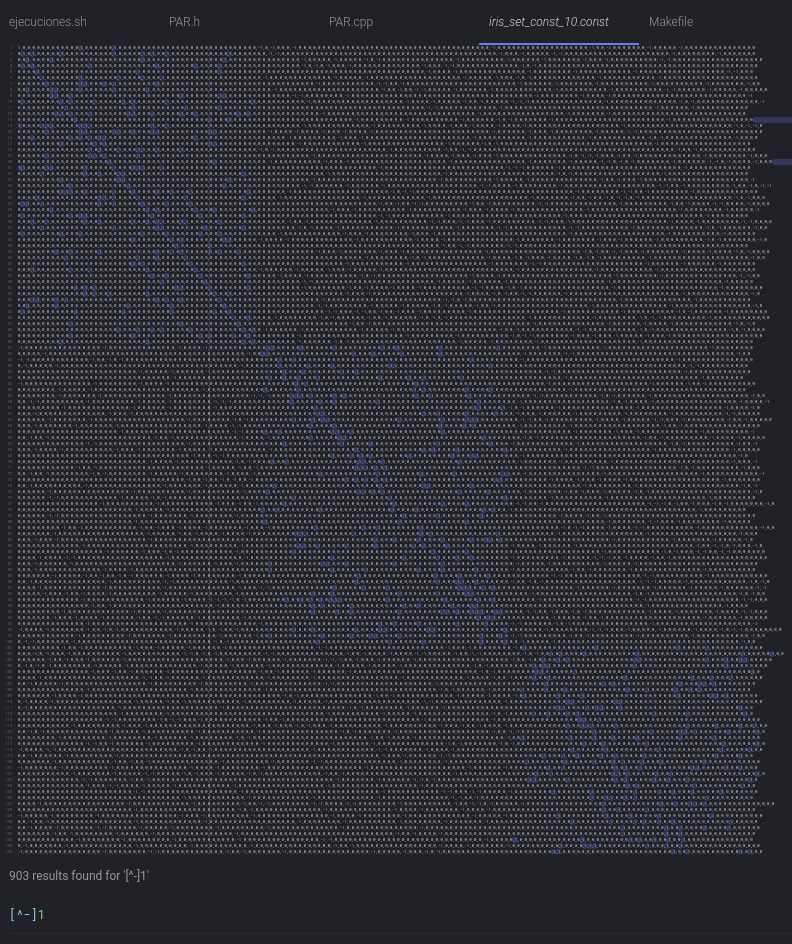
\includegraphics[scale = 0.30]{rest_iris_10.png}
 		 \caption{Ctrl+F: restricciones ML en Iris}
  		\label{fig:rest_iris_10_1}
  \end{subfigure}
  \hfill
  \begin{subfigure}[b]{0.5\textwidth}
      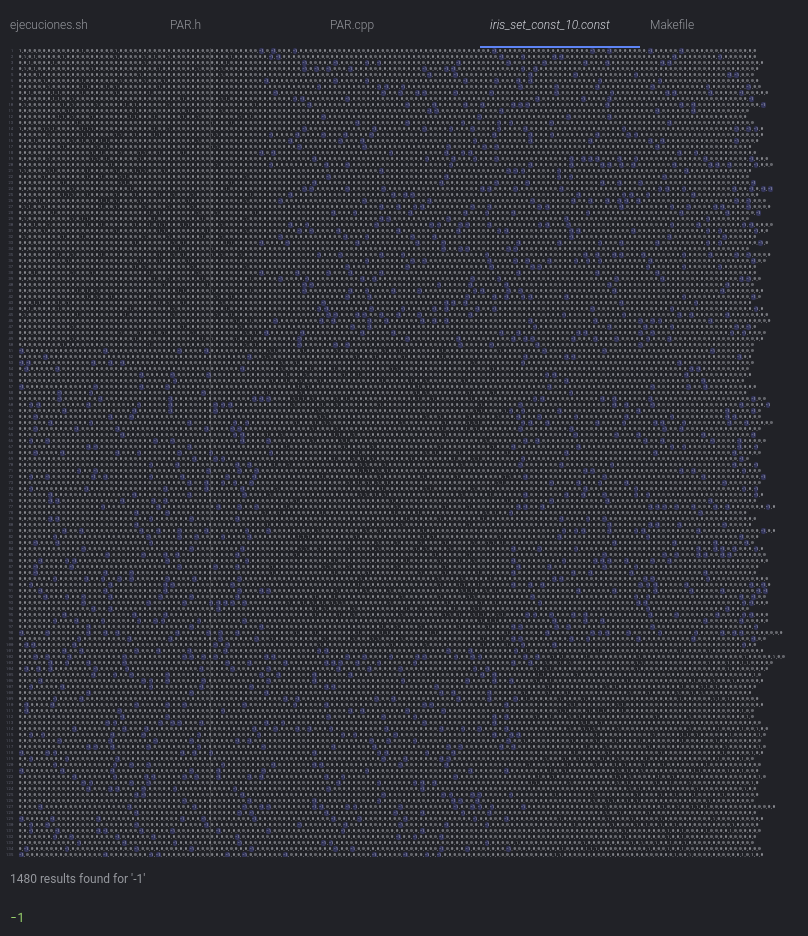
\includegraphics[scale = 0.30]{rest_iris_10_-1.png}
 		 \caption{Ctrl+F: restricciones CL en Iris}
  		\label{fig:rest_iris_10_-1}
  \end{subfigure}
    \caption{10\% de restricciones en Iris, en tono azul las coincidencias}\label{fig:rest_iris_10}

\end{figure}


\begin{figure}[H]
  \centering
  \begin{subfigure}[b]{0.45\textwidth}
      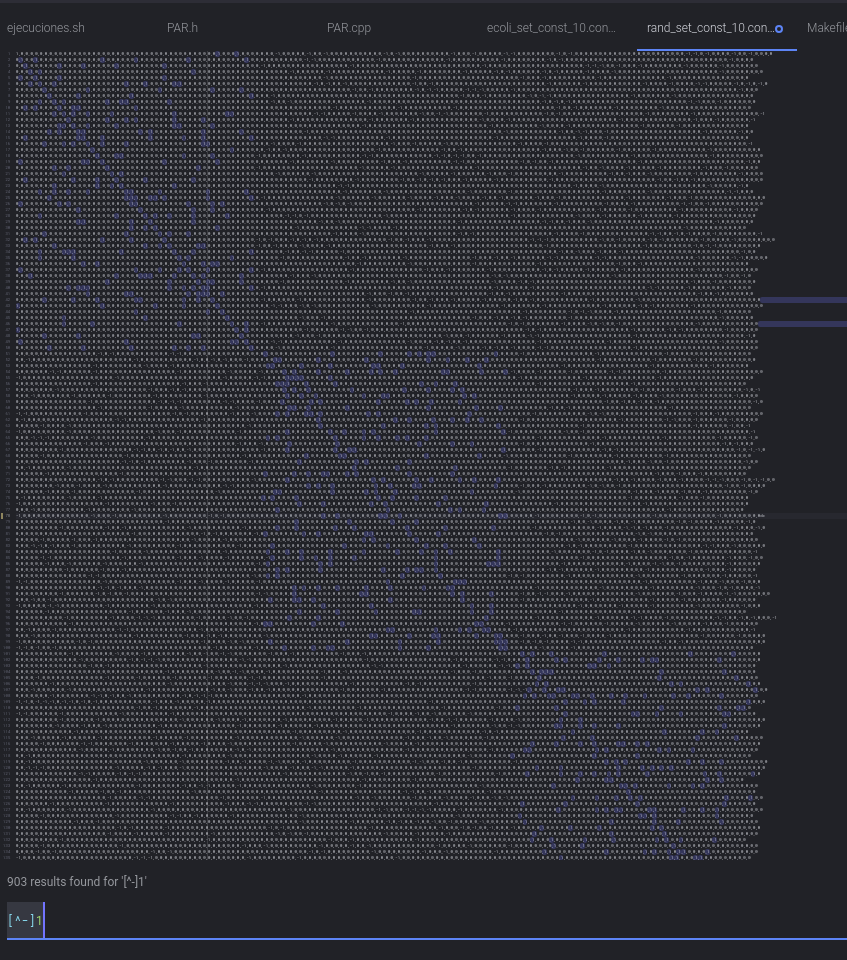
\includegraphics[scale = 0.28]{rest_rand_10.png}
 		 \caption{Ctrl+F: restricciones ML en Rand}
  		\label{fig:rest_rand_10_1}
  \end{subfigure}
  \hfill
  \begin{subfigure}[b]{0.5\textwidth}
      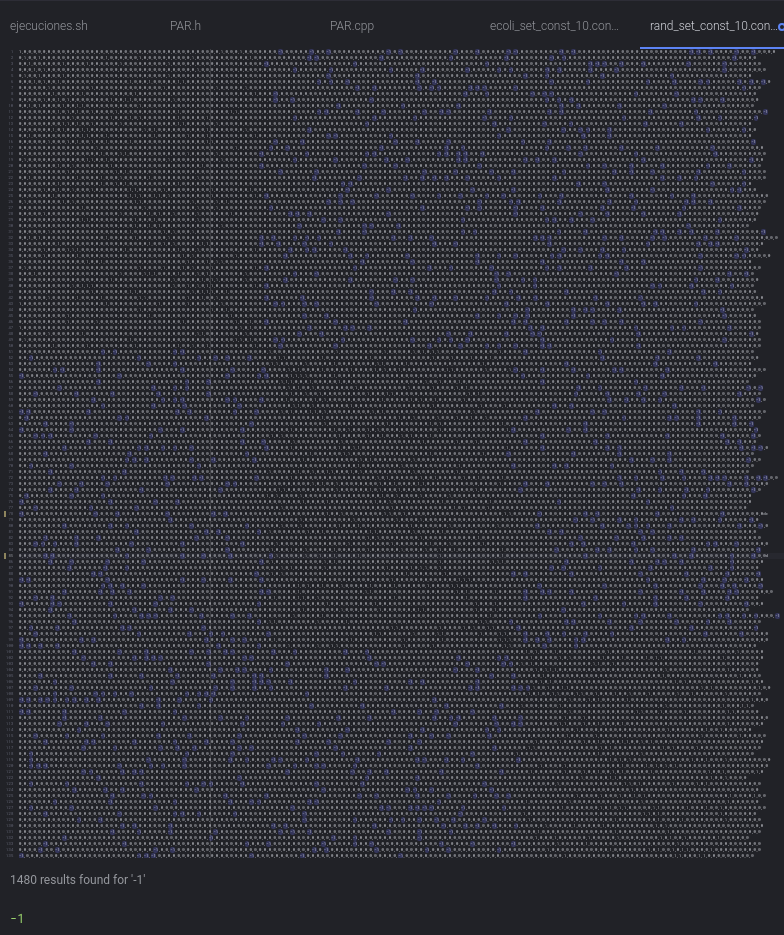
\includegraphics[scale = 0.28]{rest_rand_10_-1.png}
 		 \caption{Ctrl+F: restricciones CL en Rand}
  		\label{fig:rest_rand_10_-1}
  \end{subfigure}
    \caption{10\% de restricciones en Rand, en tono azul las coincidencias}\label{fig:rest_rand_10}

\end{figure}


\begin{figure}[H]
  \centering
  \begin{subfigure}[b]{0.55\textwidth}
     \hspace{1.2cm} 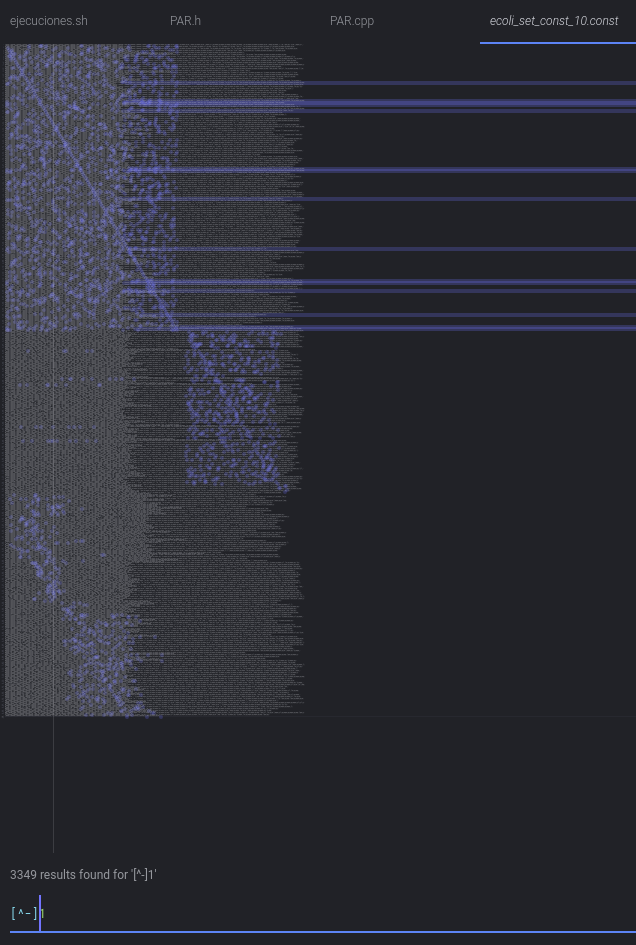
\includegraphics[scale = 0.28]{rest_ecoli_10.png}
 		 \caption{Ctrl+F: restricciones ML en Ecoli}
  		\label{fig:rest_ecoli_10_1}
  \end{subfigure}
  \hfill
  \begin{subfigure}[b]{0.40\textwidth}
      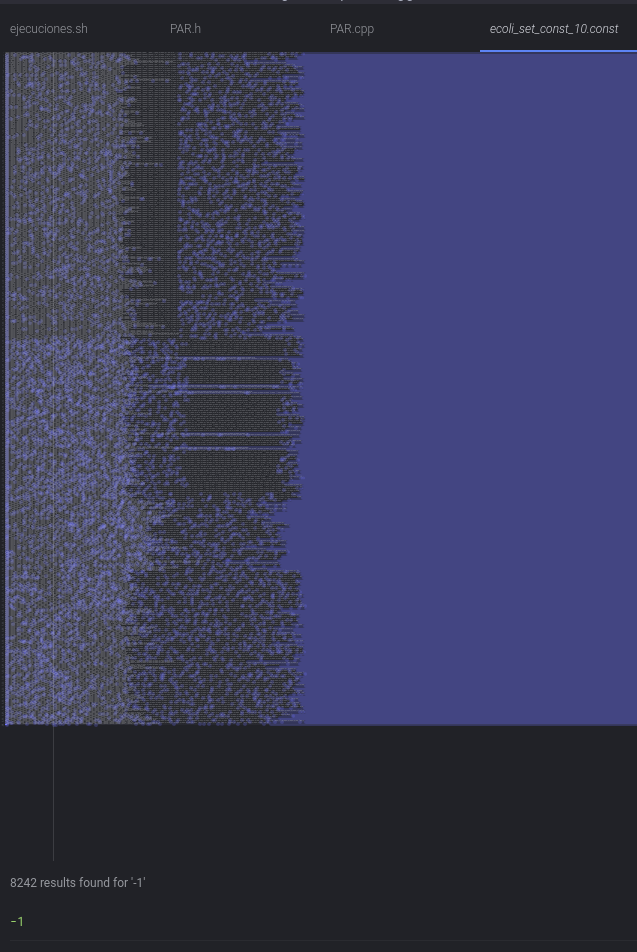
\includegraphics[scale = 0.28]{rest_ecoli_10_-1.png}
 		 \caption{Ctrl+F: restricciones CL en Ecoli}
  		\label{fig:rest_ecoli_10_-1}
  \end{subfigure}
    \caption{10\% de restricciones en Ecoli, en tono azul las coincidencias}\label{fig:rest_ecoli_10}

\end{figure}

Vemos como en Iris y Rand se aprecia totalmente que las restricciones diferenciadas para que los clusters se asignen según las propias clases del problema, mientras que en Ecoli, aunque podemos ver ciertas agrupaciones, no ocurren tanto, sobre todo con las restricciones CL.

Esto ocurre tanto en los ficheros con un 10\% de restricciones como en los ficheros con un 20\% de restricciones.

\subsubsection{Semillas escogidas.}

Uno de los problemas que encontré en el desarrollo de la práctica (comentado con los profesores) es que a veces el algoritmo Greedy ciclaba indefinidamente, ya que pasaba por una serie de soluciones y volvía a las mismas.

La forma de solucionar esto (que pasaba rara vez, pero ocurría) es buscar semillas que no ciclen ya que la secuencia de aleatorios generadas por esta asignaba los elementos que producían el ciclo a distintos clusters.

Las semillas que voy a usar son:

\begin{itemize}
	\item {123452244}
	\item {9398429}
	\item {12321}
	\item {213566}
	\item {3939021}
\end{itemize}

Estas semillas las he obtenido a base de prueba-error y comprobar que no ciclaban.

\newpage

\subsection{Resultados obtenidos.}

A continuación mostraré las tablas dadas por los profesores de la asignatura como plantilla. En las tablas de las ejecuciones explicaré el comportamiento de los algoritmos con respecto a los conjuntos de datos, mientras que en la comparación global en la sección de análisis de resultados compararé los distintos algoritmos.

\subsubsection{10\% de restricciones.}

\begin{table}[H]
\small

\begin{adjustwidth}{-1cm}{-1cm}%

\begin{tabular}{|l|c|c|c|c|c|c|c|c|c|c|c|c|}
\hline
\multicolumn{13}{|c|}{\textbf{Ejecuciones BL con un 10\% de restricciones}}                                                                                                                                                                                                                                                                                                                                            \\ \hline
\multicolumn{1}{|c|}{\multirow{2}{*}{\textbf{Semilla}}} & \multicolumn{4}{c|}{Iris}                                                                                          & \multicolumn{4}{c|}{Ecoli}                                                                                         & \multicolumn{4}{c|}{Rand}                                                                                          \\ \cline{2-13} 
\multicolumn{1}{|c|}{}                                  & \multicolumn{1}{l|}{Tasa\_C} & \multicolumn{1}{l|}{Tasa\_inf} & \multicolumn{1}{l|}{Agr.} & \multicolumn{1}{l|}{T} & \multicolumn{1}{l|}{Tasa\_C} & \multicolumn{1}{l|}{Tasa\_inf} & \multicolumn{1}{l|}{Agr.} & \multicolumn{1}{l|}{T} & \multicolumn{1}{l|}{Tasa\_C} & \multicolumn{1}{l|}{Tasa\_inf} & \multicolumn{1}{l|}{Agr.} & \multicolumn{1}{l|}{T} \\ \hline
123452244                                               & 0,60                         & 0,00                           & 0,60                      & 0,04                   & 1009,81                      & 34,00                          & 1147,55                   & 1,31                   & 0,85                         & 0,00                           & 0,85                      & 0,03                   \\ \hline
9398429                                                 & 0,60                         & 0,00                           & 0,60                      & 0,03                   & 998,07                       & 30,00                          & 1119,60                   & 1,09                   & 0,85                         & 0,00                           & 0,85                      & 0,03                   \\ \hline
12321                                                   & 0,60                         & 0,00                           & 0,60                      & 0,04                   & 1005,33                      & 36,00                          & 1151,17                   & 1,05                   & 0,85                         & 0,00                           & 0,85                      & 0,03                   \\ \hline
213566                                                  & 0,60                         & 0,00                           & 0,60                      & 0,03                   & 1025,31                      & 41,00                          & 1191,41                   & 0,93                   & 0,85                         & 0,00                           & 0,85                      & 0,03                   \\ \hline
3939021                                                 & 0,60                         & 0,00                           & 0,60                      & 0,03                   & 1038,06                      & 31,00                          & 1163,65                   & 1,01                   & 0,85                         & 0,00                           & 0,85                      & 0,03                   \\ \hline
\textbf{Media}                                          & 0,60                         & 0,00                           & 0,60                      & 0,03                   & 1015,32                      & 34,40                          & 1154,68                   & 1,08                   & 0,85                         & 0,00                           & 0,85                      & 0,03                   \\ \hline
\end{tabular}

\end{adjustwidth}

\end{table}	


% Please add the following required packages to your document preamble:
% \usepackage{multirow}
\begin{table}[H]

\small

\begin{adjustwidth}{-1cm}{-1cm}%

\begin{tabular}{|l|c|c|c|c|c|c|c|c|c|c|c|c|}
\hline
\multicolumn{13}{|c|}{\textbf{Ejecuciones Greedy con un 10\% de restricciones}}                                                                                                                                                                                                                                                                                                                                        \\ \hline
\multicolumn{1}{|c|}{\multirow{2}{*}{\textbf{Semilla}}} & \multicolumn{4}{c|}{Iris}                                                                                          & \multicolumn{4}{c|}{Ecoli}                                                                                         & \multicolumn{4}{c|}{Rand}                                                                                          \\ \cline{2-13} 
\multicolumn{1}{|c|}{}                                  & \multicolumn{1}{l|}{Tasa\_C} & \multicolumn{1}{l|}{Tasa\_inf} & \multicolumn{1}{l|}{Agr.} & \multicolumn{1}{l|}{T} & \multicolumn{1}{l|}{Tasa\_C} & \multicolumn{1}{l|}{Tasa\_inf} & \multicolumn{1}{l|}{Agr.} & \multicolumn{1}{l|}{T} & \multicolumn{1}{l|}{Tasa\_C} & \multicolumn{1}{l|}{Tasa\_inf} & \multicolumn{1}{l|}{Agr.} & \multicolumn{1}{l|}{T} \\ \hline
123452244                                               & 0,60                         & 7,00                           & 0,91                      & 0,02                   & 1596,56                      & 408,00                         & 3249,44                   & 0,23                   & 0,85                         & 0,00                           & 0,85                      & 0,01                   \\ \hline
9398429                                                 & 0,60                         & 47,00                          & 2,71                      & 0,01                   & 1584,45                      & 256,00                         & 2621,55                   & 0,29                   & 0,85                         & 0,00                           & 0,85                      & 0,01                   \\ \hline
12321                                                   & 0,60                         & 30,00                          & 1,95                      & 0,01                   & 1613,80                      & 172,00                         & 2310,60                   & 0,48                   & 0,85                         & 0,00                           & 0,85                      & 0,01                   \\ \hline
213566                                                  & 0,60                         & 0,00                           & 0,60                      & 0,01                   & 1584,23                      & 95,00                          & 1969,09                   & 0,28                   & 0,85                         & 0,00                           & 0,85                      & 0,00                   \\ \hline
3939021                                                 & 0,60                         & 7,00                           & 0,91                      & 0,01                   & 1722,98                      & 195,00                         & 2512,96                   & 0,38                   & 0,85                         & 0,00                           & 0,85                      & 0,00                   \\ \hline
\textbf{Media}                                          & 0,60                         & 18,20                          & 1,42                      & 0,01                   & 1620,40                      & 225,20                         & 2532,73                   & 0,33                   & 0,85                         & 0,00                           & 0,85                      & 0,01                   \\ \hline
\end{tabular}

\end{adjustwidth}

\end{table}


Vemos como efectivamente, con lo comentado anteriormente, tanto Iris como Rand obtienen un valor muy bueno, que como podemos comprobar en la asignación de elementos en los ficheros de salida del programa, son las asignaciones óptimas para el problema de asignación clásico, sin embargo Ecoli, que si tiene aleatoriedad en su fichero de restricciones si necesita incumplir restricciones para realizar las asignaciones, llegando a veces a dejar clusters con un único elemento como podemos observar en los ficheros de salida del programa, ya que por las restricciones no es capaz de formar un cluster completo sin aumentar la función objetivo.

Con respecto a la tabla de BL podemos observar que tanto para Iris como para Rand llegamos a la misma solución independientemente de la semilla utilizada, lo que nos indica que en esos puntos existe un mínimo para ese conjunto de datos, aunque utilizando búsqueda local nunca podemos asegurar que ese mínimo sea el optimo. Ecoli sin embargo si tenemos más variedad de soluciones, viendo un equilibro entre la desviación general y la tasa de infactibilidad entre los valores 998 y 1040 y valores entre 30 y 40, respectivamente. Esto nos hace entender mejor como trabaja la función objetivo, ya que intenta equilibrar estos dos valores para intentar minimizar ambos, seguiré comentado esto en la sección de experimentos.

Con respecto a la tabla del algoritmo Greedy vemos como esta vez en Iris, aunque mantiene la desviación general al mismo nivel que búsqueda local, no es capaz de mantener una baja infactibilidad por lo ya comentado de la gestión de restricciones. En Rand este algoritmo si es capaz de llegar a la misma solución que BL, seguramente por lo comentado del fichero de restricciones. De cara a Ecoli podemos ver que tanto la desviación general como la infactibilidad es mucho más inestable, ya que depende de la \"suerte\" que tenga el algoritmo con la semilla aleatoria y el orden de los elementos, para que estos no generen grandes tasas de incumplimiento de restricciones y permita agrupar a los elementos de una forma más coherente.

\subsubsection{20\% de restricciones.}

\begin{table}[H]

\small

\begin{adjustwidth}{-1cm}{-1cm}%


\begin{tabular}{|l|c|c|c|c|c|c|c|c|c|c|c|c|}
\hline
\multicolumn{13}{|c|}{\textbf{Ejecuciones BL con un 20\% de restricciones}}                                                                                                                                                                                                                                                                                                                                            \\ \hline
\multicolumn{1}{|c|}{\multirow{2}{*}{\textbf{Semilla}}} & \multicolumn{4}{c|}{Iris}                                                                                          & \multicolumn{4}{c|}{Ecoli}                                                                                         & \multicolumn{4}{c|}{Rand}                                                                                          \\ \cline{2-13} 
\multicolumn{1}{|c|}{}                                  & \multicolumn{1}{l|}{Tasa\_C} & \multicolumn{1}{l|}{Tasa\_inf} & \multicolumn{1}{l|}{Agr.} & \multicolumn{1}{l|}{T} & \multicolumn{1}{l|}{Tasa\_C} & \multicolumn{1}{l|}{Tasa\_inf} & \multicolumn{1}{l|}{Agr.} & \multicolumn{1}{l|}{T} & \multicolumn{1}{l|}{Tasa\_C} & \multicolumn{1}{l|}{Tasa\_inf} & \multicolumn{1}{l|}{Agr.} & \multicolumn{1}{l|}{T} \\ \hline
123452244                                               & 0,60                         & 0,00                           & 0,60                      & 0,03                   & 1003,50                      & 77,00                          & 1159,47                   & 1,52                   & 0,85                         & 0,00                           & 0,85                      & 0,03                   \\ \hline
9398429                                                 & 0,60                         & 0,00                           & 0,60                      & 0,05                   & 1034,73                      & 85,00                          & 1206,90                   & 1,17                   & 0,85                         & 0,00                           & 0,85                      & 0,03                   \\ \hline
12321                                                   & 0,60                         & 0,00                           & 0,60                      & 0,04                   & 975,78                       & 87,00                          & 1152,01                   & 1,26                   & 0,85                         & 0,00                           & 0,85                      & 0,03                   \\ \hline
213566                                                  & 0,60                         & 0,00                           & 0,60                      & 0,03                   & 1020,51                      & 99,00                          & 1221,04                   & 1,12                   & 0,85                         & 0,00                           & 0,85                      & 0,03                   \\ \hline
3939021                                                 & 0,60                         & 0,00                           & 0,60                      & 0,03                   & 982,74                       & 118,00                         & 1221,76                   & 1,38                   & 0,85                         & 0,00                           & 0,85                      & 0,03                   \\ \hline
\textbf{Media}                                          & 0,60                         & 0,00                           & 0,60                      & 0,04                   & 1003,45                      & 93,20                          & 1192,24                   & 1,29                   & 0,85                         & 0,00                           & 0,85                      & 0,03                   \\ \hline
\end{tabular}
\end{adjustwidth}

\end{table}




\begin{table}[H]
\small

\begin{adjustwidth}{-1cm}{-1cm}%

\begin{tabular}{|l|c|c|c|c|c|c|c|c|c|c|c|c|}
\hline
\multicolumn{13}{|c|}{\textbf{Ejecuciones Greedy con un 20\% de restricciones}}                                                                                                                                                                                                                                                                                                                                        \\ \hline
\multicolumn{1}{|c|}{\multirow{2}{*}{\textbf{Semilla}}} & \multicolumn{4}{c|}{Iris}                                                                                          & \multicolumn{4}{c|}{Ecoli}                                                                                         & \multicolumn{4}{c|}{Rand}                                                                                          \\ \cline{2-13} 
\multicolumn{1}{|c|}{}                                  & \multicolumn{1}{l|}{Tasa\_C} & \multicolumn{1}{l|}{Tasa\_inf} & \multicolumn{1}{l|}{Agr.} & \multicolumn{1}{l|}{T} & \multicolumn{1}{l|}{Tasa\_C} & \multicolumn{1}{l|}{Tasa\_inf} & \multicolumn{1}{l|}{Agr.} & \multicolumn{1}{l|}{T} & \multicolumn{1}{l|}{Tasa\_C} & \multicolumn{1}{l|}{Tasa\_inf} & \multicolumn{1}{l|}{Agr.} & \multicolumn{1}{l|}{T} \\ \hline
123452244                                               & 0,87                         & 69,00                          & 2,42                      & 0,01                   & 1491,53                      & 307,00                         & 2113,39                   & 0,20                   & 0,85                         & 0,00                           & 0,85                      & 0,00                   \\ \hline
9398429                                                 & 0,59                         & 17,00                          & 0,97                      & 0,01                   & 1676,16                      & 282,00                         & 2247,38                   & 0,11                   & 0,85                         & 0,00                           & 0,85                      & 0,01                   \\ \hline
12321                                                   & 0,60                         & 0,00                           & 0,60                      & 0,01                   & 1440,98                      & 108,00                         & 1659,74                   & 0,53                   & 0,85                         & 0,00                           & 0,85                      & 0,01                   \\ \hline
213566                                                  & 0,60                         & 52,00                          & 1,77                      & 0,01                   & 1551,01                      & 215,00                         & 1986,51                   & 0,17                   & 0,85                         & 0,00                           & 0,85                      & 0,00                   \\ \hline
3939021                                                 & 0,59                         & 17,00                          & 0,98                      & 0,01                   & 1470,86                      & 191,00                         & 1857,75                   & 0,27                   & 0,85                         & 0,00                           & 0,85                      & 0,01                   \\ \hline
\textbf{Media}                                          & 0,65                         & 31,00                          & 1,35                      & 0,01                   & 1526,11                      & 220,60                         & 1972,95                   & 0,25                   & 0,85                         & 0,00                           & 0,85                      & 0,01                   \\ \hline
\end{tabular}

\end{adjustwidth}

\end{table}

En general, podemos ver que se mantiene lo dicho con un 10\% de restricciones, a continuación comentaré los cambios más remarcables.

En búsqueda local vemos como se repite la situación, tanto en Iris como en Rand el aumento de restricciones no impide volver a tener la misma solución que con un 10\% de restricciones, ya que estos ficheros tienen la misma disposición de las restricciones. De nuevo, en el caso de Ecoli ocurre la misma situación, vemos como mantiene cierto equilibro gracias a la forma de la función objetivo, sin embargo se ve obligado a incumplir más restricciones por el aumento del porcentaje.

En el caso de greedy para Rand vuelve a ocurrir lo mismo, mientras que para Iris si existen ciertos cambios, vemos como es capaz de mejorar el valor de algunas desviaciones generales, pero esto es debido a que por las restricciones decide dejar clusters un poco más vacios, acercando los elementos que están dentro, eso sí, aumentando la tasa de restricciones incumplidas.

\newpage


\subsection{Análisis de resultados.	}

A continuación podemos ver la media de las distintas ejecuciones, tanto para un 10\% de restricciones como para un 20\%:



\begin{table}[H]
\small
\begin{adjustwidth}{-1cm}{-1cm}%


\begin{tabular}{|c|c|c|c|c|c|c|c|c|c|c|c|c|}
\hline
\multicolumn{13}{|c|}{\textbf{Resultados globales en el PAR con 10\% de restricciones}}                                                                                                                                                                                                                                                                                                              \\ \hline
\multirow{2}{*}{\textbf{Algoritmo}}   & \multicolumn{4}{c|}{Iris}                                                                                          & \multicolumn{4}{c|}{Ecoli}                                                                                         & \multicolumn{4}{c|}{Rand}                                                                                          \\ \cline{2-13} 
                                      & \multicolumn{1}{l|}{Tasa\_C} & \multicolumn{1}{l|}{Tasa\_inf} & \multicolumn{1}{l|}{Agr.} & \multicolumn{1}{l|}{T} & \multicolumn{1}{l|}{Tasa\_C} & \multicolumn{1}{l|}{Tasa\_inf} & \multicolumn{1}{l|}{Agr.} & \multicolumn{1}{l|}{T} & \multicolumn{1}{l|}{Tasa\_C} & \multicolumn{1}{l|}{Tasa\_inf} & \multicolumn{1}{l|}{Agr.} & \multicolumn{1}{l|}{T} \\ \hline
\multicolumn{1}{|l|}{\textbf{Greedy}} & 0,60                         & 18,20                          & 1,42                      & 0,01                   & 1620,40                      & 225,20                         & 2532,73                   & 0,33                   & 0,85                         & 0,00                           & 0,85                      & 0,01                   \\ \hline
\multicolumn{1}{|l|}{\textbf{BL}}     & 0,60                         & 0,00                           & 0,60                      & 0,03                   & 1015,32                      & 34,40                          & 1154,68                   & 1,08                   & 0,85                         & 0,00                           & 0,85                      & 0,03                   \\ \hline
\end{tabular}

\end{adjustwidth}
\end{table}




\begin{table}[H]
\small
\begin{adjustwidth}{-1cm}{-1cm}%


\begin{tabular}{|c|c|c|c|c|c|c|c|c|c|c|c|c|}
\hline
\multicolumn{13}{|c|}{\textbf{Resultados globales en el PAR con 20\% de restricciones}}                                                                                                                                                                                                                                                                                                              \\ \hline
\multirow{2}{*}{\textbf{Algoritmo}}   & \multicolumn{4}{c|}{Iris}                                                                                          & \multicolumn{4}{c|}{Ecoli}                                                                                         & \multicolumn{4}{c|}{Rand}                                                                                          \\ \cline{2-13} 
                                      & \multicolumn{1}{l|}{Tasa\_C} & \multicolumn{1}{l|}{Tasa\_inf} & \multicolumn{1}{l|}{Agr.} & \multicolumn{1}{l|}{T} & \multicolumn{1}{l|}{Tasa\_C} & \multicolumn{1}{l|}{Tasa\_inf} & \multicolumn{1}{l|}{Agr.} & \multicolumn{1}{l|}{T} & \multicolumn{1}{l|}{Tasa\_C} & \multicolumn{1}{l|}{Tasa\_inf} & \multicolumn{1}{l|}{Agr.} & \multicolumn{1}{l|}{T} \\ \hline
\multicolumn{1}{|l|}{\textbf{Greedy}} & 0,65                         & 31,00                          & 1,35                      & 0,01                   & 1526,11                      & 220,60                         & 1972,95                   & 0,25                   & 0,85                         & 0,00                           & 0,85                      & 0,01                   \\ \hline
\multicolumn{1}{|l|}{\textbf{BL}}     & 0,60                         & 0,00                           & 0,60                      & 0,04                   & 1003,45                      & 93,20                          & 1192,24                   & 1,29                   & 0,85                         & 0,00                           & 0,85                      & 0,03                   \\ \hline
\end{tabular}

\end{adjustwidth}
\end{table}


En este resumen en el que vemos las medias de las distintas ejecuciones para los distintos algoritmos, tanto con un 10\% de restricciones como con un 20\% de restricciones.

Podemos observar como el algoritmo de búsqueda local se comporta bastante mejor que el algoritmo greedy, tanto en minimizar la desviación general como en minimizar el número de restricciones incumplidas. Esto se da por lo ya comentado para el algoritmo greedy sobre el aumento de restricciones incumplidas, que es incapaz de volver atrás al colocar un elemento y tampoco tiene en cuenta los elementos que introducirá en los clusters.

Este problema no lo observamos en el algoritmo de búsqueda local, ya que la evaluación y selección del vecino penaliza el incumplir restricciones y siempre trabajamos con el total de restricciones incumplidas, no con el de una solución parcial como en el algoritmo greedy.

Con respecto al tiempo, el algoritmo de búsqueda local es considerablemente más lento, en todos los casos, aunque sus tiempos de ejecución siguen dentro de lo razonable, dando resultados prácticamente inmediatos, aunque en peor tiempo que Greedy. Esto no quita que aunque sea un poco más lento, esto apenas es apreciable ya que todos los tiempos están por debajo de los 1,3 segundos, y aun así el valor de la función objetivo es mucho más bajo en búsqueda local.

Como tanto la desviación general como en la infactibilidad conseguimos mejores resultados con búsqueda local, la agregación total es menor, por lo que consideramos mejores las soluciones tanto con un 10 como con un 20 por ciento de restricciones. La única excepción es para el conjunto de datos Rand, ya que obtenemos la misma solución con greedy y con BL, pero el tiempo de greedy es menor, por lo que podemos considerar en este caso greedy como un mejor algoritmo.

También comentar que el hecho de factorizar los algoritmos ha permitido ejecutarlos en un tiempo más que razonable (unos 20 segundos para las 30 ejecuciones), mientras que sin factorizar llegaba a tardar unos 15 minutos para las 30 ejecuciones del algoritmo.


\newpage

\subsection{Otros experimentos realizados.}

\subsubsection{Modificación de la función objetivo}

Hemos visto que pasaría con la siguiente función objetivo:

$$ \lambda = \frac{D_{max}}{NumRestricciones} $$ 

$$ f = C + (\textit{Infeasibility} * \lambda) $$ 

Sin embargo, he probado a modificar el valor de $\lambda$, de forma que la penalización por incumplir restricciones sea mucho mayor para intentar minimizar lo máximo posible la tasa de \textit{infeasibility}:


$$ \lambda = \frac{D_{max}^2}{NumRestricciones} $$ 

$$ f = C + (\textit{Infeasibility} * \lambda) $$ 



Con esto hemos obteniendo los siguientes resultados:

\begin{table}[H]
\small

\begin{adjustwidth}{-1.2cm}{-1.2cm}%

\begin{tabular}{|l|c|c|c|c|c|c|c|c|c|c|c|c|}
\hline
\multicolumn{13}{|c|}{\textbf{Ejecuciones BL con un 10\% de restricciones penalizando restricciones}}                                                                                                                                                                                                                                                                                                                  \\ \hline
\multicolumn{1}{|c|}{\multirow{2}{*}{\textbf{Semilla}}} & \multicolumn{4}{c|}{Iris}                                                                                          & \multicolumn{4}{c|}{Ecoli}                                                                                         & \multicolumn{4}{c|}{Rand}                                                                                          \\ \cline{2-13} 
\multicolumn{1}{|c|}{}                                  & \multicolumn{1}{l|}{Tasa\_C} & \multicolumn{1}{l|}{Tasa\_inf} & \multicolumn{1}{l|}{Agr.} & \multicolumn{1}{l|}{T} & \multicolumn{1}{l|}{Tasa\_C} & \multicolumn{1}{l|}{Tasa\_inf} & \multicolumn{1}{l|}{Agr.} & \multicolumn{1}{l|}{T} & \multicolumn{1}{l|}{Tasa\_C} & \multicolumn{1}{l|}{Tasa\_inf} & \multicolumn{1}{l|}{Agr.} & \multicolumn{1}{l|}{T} \\ \hline
123452244                                               & 0,60                         & 0,00                           & 0,60                      & 0,04                   & 1657,33                      & 36,00                          & 3326859,89                & 1,34                   & 0,85                         & 0,00                           & 0,85                      & 0,03                   \\ \hline
9398429                                                 & 0,60                         & 0,00                           & 0,60                      & 0,03                   & 1491,50                      & 21,00                          & 1941192,99                & 1,67                   & 0,85                         & 0,00                           & 0,85                      & 0,03                   \\ \hline
12321                                                   & 0,60                         & 0,00                           & 0,60                      & 0,04                   & 1423,07                      & 1,00                           & 93789,81                  & 1,51                   & 0,85                         & 0,00                           & 0,85                      & 0,03                   \\ \hline
213566                                                  & 0,60                         & 0,00                           & 0,60                      & 0,03                   & 1547,14                      & 9,00                           & 832847,78                 & 1,22                   & 0,85                         & 0,00                           & 0,85                      & 0,03                   \\ \hline
3939021                                                 & 0,60                         & 0,00                           & 0,60                      & 0,03                   & 1533,86                      & 12,00                          & 1109934,71                & 1,27                   & 0,85                         & 0,00                           & 0,85                      & 0,03                   \\ \hline
\textbf{Media}                                          & 0,60                         & 0,00                           & 0,60                      & 0,03                   & 1530,58                      & 15,80                          & 1460925,04                & 1,40                   & 0,85                         & 0,00                           & 0,85                      & 0,03                   \\ \hline
\end{tabular}

\end{adjustwidth}

\end{table}

\begin{table}[H]
\small

\begin{adjustwidth}{-1.2cm}{-1.2cm}%

\begin{tabular}{|l|c|c|c|c|c|c|c|c|c|c|c|c|}
\hline
\multicolumn{13}{|c|}{\textbf{Ejecuciones BL con un 20\% de restricciones penalizando restricciones}}                                                                                                                                                                                                                                                                                                                  \\ \hline
\multicolumn{1}{|c|}{\multirow{2}{*}{\textbf{Semilla}}} & \multicolumn{4}{c|}{Iris}                                                                                          & \multicolumn{4}{c|}{Ecoli}                                                                                         & \multicolumn{4}{c|}{Rand}                                                                                          \\ \cline{2-13} 
\multicolumn{1}{|c|}{}                                  & \multicolumn{1}{l|}{Tasa\_C} & \multicolumn{1}{l|}{Tasa\_inf} & \multicolumn{1}{l|}{Agr.} & \multicolumn{1}{l|}{T} & \multicolumn{1}{l|}{Tasa\_C} & \multicolumn{1}{l|}{Tasa\_inf} & \multicolumn{1}{l|}{Agr.} & \multicolumn{1}{l|}{T} & \multicolumn{1}{l|}{Tasa\_C} & \multicolumn{1}{l|}{Tasa\_inf} & \multicolumn{1}{l|}{Agr.} & \multicolumn{1}{l|}{T} \\ \hline
123452244                                               & 0,60                         & 0,00                           & 0,60                      & 0,03                   & 1273,62                      & 0,00                           & 1273,62                   & 1,52                   & 0,85                         & 0,00                           & 0,85                      & 0,03                   \\ \hline
9398429                                                 & 0,60                         & 0,00                           & 0,60                      & 0,05                   & 1093,38                      & 0,00                           & 1093,38                   & 1,60                   & 0,85                         & 0,00                           & 0,85                      & 0,03                   \\ \hline
12321                                                   & 0,60                         & 0,00                           & 0,60                      & 0,04                   & 1093,38                      & 0,00                           & 1093,38                   & 1,67                   & 0,85                         & 0,00                           & 0,85                      & 0,03                   \\ \hline
213566                                                  & 0,60                         & 0,00                           & 0,60                      & 0,03                   & 1274,84                      & 0,00                           & 1274,84                   & 2,03                   & 0,85                         & 0,00                           & 0,85                      & 0,03                   \\ \hline
3939021                                                 & 0,60                         & 0,00                           & 0,60                      & 0,03                   & 1274,84                      & 0,00                           & 1274,84                   & 1,46                   & 0,85                         & 0,00                           & 0,85                      & 0,03                   \\ \hline
\textbf{Media}                                          & 0,60                         & 0,00                           & 0,60                      & 0,04                   & 1202,01                      & 0,00                           & 1202,01                   & 1,66                   & 0,85                         & 0,00                           & 0,85                      & 0,03                   \\ \hline
\end{tabular}
\end{adjustwidth}

\end{table}

\newpage

También he probado el caso contrario, es decir, apenas penalizar el incumplir las restricciones: 

$$ \lambda = \frac{D_{max}}{NumRestricciones^2} $$ 

$$ f = C + (\textit{Infeasibility} * \lambda) $$ 

Obteniendo los siguientes resultados:


\begin{table}[H]
\small

\begin{adjustwidth}{-1cm}{-1cm}%

\begin{tabular}{|l|c|c|c|c|c|c|c|c|c|c|c|c|}
\hline
\multicolumn{13}{|c|}{\textbf{Ejecuciones BL con un 10\% de restricciones NO penalizando restricciones}}                                                                                                                                                                                                                                                                                                               \\ \hline
\multicolumn{1}{|c|}{\multirow{2}{*}{\textbf{Semilla}}} & \multicolumn{4}{c|}{Iris}                                                                                          & \multicolumn{4}{c|}{Ecoli}                                                                                         & \multicolumn{4}{c|}{Rand}                                                                                          \\ \cline{2-13} 
\multicolumn{1}{|c|}{}                                  & \multicolumn{1}{l|}{Tasa\_C} & \multicolumn{1}{l|}{Tasa\_inf} & \multicolumn{1}{l|}{Agr.} & \multicolumn{1}{l|}{T} & \multicolumn{1}{l|}{Tasa\_C} & \multicolumn{1}{l|}{Tasa\_inf} & \multicolumn{1}{l|}{Agr.} & \multicolumn{1}{l|}{T} & \multicolumn{1}{l|}{Tasa\_C} & \multicolumn{1}{l|}{Tasa\_inf} & \multicolumn{1}{l|}{Agr.} & \multicolumn{1}{l|}{T} \\ \hline
123452244                                               & 0,52                         & 139,00                         & 0,53                      & 0,04                   & 303,78                       & 4080,00                        & 303,82                    & 1,38                   & 0,84                         & 11,00                          & 0,84                      & 0,03                   \\ \hline
9398429                                                 & 0,52                         & 182,00                         & 0,52                      & 0,04                   & 303,67                       & 4050,00                        & 303,71                    & 1,66                   & 0,84                         & 11,00                          & 0,84                      & 0,03                   \\ \hline
12321                                                   & 0,52                         & 182,00                         & 0,52                      & 0,06                   & 303,77                       & 4033,00                        & 303,81                    & 1,63                   & 0,84                         & 11,00                          & 0,84                      & 0,03                   \\ \hline
213566                                                  & 0,52                         & 139,00                         & 0,53                      & 0,05                   & 302,82                       & 4045,00                        & 302,86                    & 1,58                   & 0,84                         & 11,00                          & 0,84                      & 0,03                   \\ \hline
3939021                                                 & 0,52                         & 139,00                         & 0,53                      & 0,04                   & 303,26                       & 4082,00                        & 303,30                    & 1,84                   & 0,84                         & 11,00                          & 0,84                      & 0,03                   \\ \hline
\textbf{Media}                                          & 0,52                         & 156,20                         & 0,53                      & 0,05                   & 303,46                       & 4058,00                        & 303,50                    & 1,62                   & 0,84                         & 11,00                          & 0,84                      & 0,03                   \\ \hline
\end{tabular}
\end{adjustwidth}

\end{table}


\begin{table}[H]
\small

\begin{adjustwidth}{-1cm}{-1cm}%

\begin{tabular}{|l|c|c|c|c|c|c|c|c|c|c|c|c|}
\hline
\multicolumn{13}{|c|}{\textbf{Ejecuciones BL con un 20\% de restricciones NO penalizando restricciones}}                                                                                                                                                                                                                                                                                                               \\ \hline
\multicolumn{1}{|c|}{\multirow{2}{*}{\textbf{Semilla}}} & \multicolumn{4}{c|}{Iris}                                                                                          & \multicolumn{4}{c|}{Ecoli}                                                                                         & \multicolumn{4}{c|}{Rand}                                                                                          \\ \cline{2-13} 
\multicolumn{1}{|c|}{}                                  & \multicolumn{1}{l|}{Tasa\_C} & \multicolumn{1}{l|}{Tasa\_inf} & \multicolumn{1}{l|}{Agr.} & \multicolumn{1}{l|}{T} & \multicolumn{1}{l|}{Tasa\_C} & \multicolumn{1}{l|}{Tasa\_inf} & \multicolumn{1}{l|}{Agr.} & \multicolumn{1}{l|}{T} & \multicolumn{1}{l|}{Tasa\_C} & \multicolumn{1}{l|}{Tasa\_inf} & \multicolumn{1}{l|}{Agr.} & \multicolumn{1}{l|}{T} \\ \hline
123452244                                               & 0,52                         & 374,00                         & 0,52                      & 0,07                   & 303,82                       & 8107,00                        & 303,90                    & 2,12                   & 0,84                         & 18,00                          & 0,84                      & 0,03                   \\ \hline
9398429                                                 & 0,52                         & 374,00                         & 0,52                      & 0,04                   & 303,69                       & 8125,00                        & 303,77                    & 1,93                   & 0,84                         & 18,00                          & 0,84                      & 0,03                   \\ \hline
12321                                                   & 0,52                         & 374,00                         & 0,52                      & 0,05                   & 303,56                       & 8133,00                        & 303,64                    & 2,02                   & 0,84                         & 18,00                          & 0,84                      & 0,03                   \\ \hline
213566                                                  & 0,52                         & 257,00                         & 0,52                      & 0,06                   & 302,83                       & 8134,00                        & 302,91                    & 2,34                   & 0,84                         & 18,00                          & 0,84                      & 0,03                   \\ \hline
3939021                                                 & 0,52                         & 257,00                         & 0,52                      & 0,05                   & 303,52                       & 8191,00                        & 303,60                    & 2,77                   & 0,84                         & 18,00                          & 0,84                      & 0,03                   \\ \hline
\textbf{Media}                                          & 0,52                         & 327,20                         & 0,52                      & 0,05                   & 303,48                       & 8138,00                        & 303,56                    & 2,24                   & 0,84                         & 18,00                          & 0,84                      & 0,03                   \\ \hline
\end{tabular}
\end{adjustwidth}

\end{table}

\newpage

Comentaré el resumen de ambas tablas:

\begin{table}[H]
\small
\begin{adjustwidth}{-2cm}{-2cm}%


\begin{tabular}{|l|c|c|c|c|c|c|c|c|c|c|c|c|}
\hline
\multicolumn{13}{|c|}{\textbf{Resultados globales con un 10\% de restricciones}}                                                                                                                                                                                                                                                                                                                                       \\ \hline
\multicolumn{1}{|c|}{\multirow{2}{*}{\textbf{Semilla}}} & \multicolumn{4}{c|}{Iris}                                                                                          & \multicolumn{4}{c|}{Ecoli}                                                                                         & \multicolumn{4}{c|}{Rand}                                                                                          \\ \cline{2-13} 
\multicolumn{1}{|c|}{}                                  & \multicolumn{1}{l|}{Tasa\_C} & \multicolumn{1}{l|}{Tasa\_inf} & \multicolumn{1}{l|}{Agr.} & \multicolumn{1}{l|}{T} & \multicolumn{1}{l|}{Tasa\_C} & \multicolumn{1}{l|}{Tasa\_inf} & \multicolumn{1}{l|}{Agr.} & \multicolumn{1}{l|}{T} & \multicolumn{1}{l|}{Tasa\_C} & \multicolumn{1}{l|}{Tasa\_inf} & \multicolumn{1}{l|}{Agr.} & \multicolumn{1}{l|}{T} \\ \hline
Greedy                                                  & 0,60                         & 18,20                          & 1,42                      & 0,01                   & 1620,40                      & 225,20                         & 2532,73                   & 0,33                   & 0,85                         & 0,00                           & 0,85                      & 0,01                   \\ \hline
BL                                                      & 0,60                         & 0,00                           & 0,60                      & 0,03                   & 1015,32                      & 34,40                          & 1154,68                   & 1,08                   & 0,85                         & 0,00                           & 0,85                      & 0,03                   \\ \hline
BL\_Cumple\_rest                                        & 0,60                         & 0,00                           & 0,60                      & 0,03                   & 1530,58                      & 15,80                          & 1460925,04                & 1,40                   & 0,85                         & 0,00                           & 0,85                      & 0,03                   \\ \hline
BL\_incumple\_rest                                      & 0,52                         & 156,20                         & 0,53                      & 0,05                   & 303,46                       & 4058,00                        & 303,50                    & 1,62                   & 0,84                         & 11,00                          & 0,84                      & 0,03                  \\ \hline
\end{tabular}

\end{adjustwidth}
\end{table}


\begin{table}[H]
\small
\begin{adjustwidth}{-1.9cm}{-1.9cm}%


\begin{tabular}{|l|c|c|c|c|c|c|c|c|c|c|c|c|}
\hline
\multicolumn{13}{|c|}{\textbf{Resultados globales con un 20\% de restricciones}}                                                                                                                                                                                                                                                                                                                                       \\ \hline
\multicolumn{1}{|c|}{\multirow{2}{*}{\textbf{Semilla}}} & \multicolumn{4}{c|}{Iris}                                                                                          & \multicolumn{4}{c|}{Ecoli}                                                                                         & \multicolumn{4}{c|}{Rand}                                                                                          \\ \cline{2-13} 
\multicolumn{1}{|c|}{}                                  & \multicolumn{1}{l|}{Tasa\_C} & \multicolumn{1}{l|}{Tasa\_inf} & \multicolumn{1}{l|}{Agr.} & \multicolumn{1}{l|}{T} & \multicolumn{1}{l|}{Tasa\_C} & \multicolumn{1}{l|}{Tasa\_inf} & \multicolumn{1}{l|}{Agr.} & \multicolumn{1}{l|}{T} & \multicolumn{1}{l|}{Tasa\_C} & \multicolumn{1}{l|}{Tasa\_inf} & \multicolumn{1}{l|}{Agr.} & \multicolumn{1}{l|}{T} \\ \hline
Greedy                                                  & 0,65                         & 31,00                          & 1,35                      & 0,01                   & 1526,11                      & 220,60                         & 1972,95                   & 0,25                   & 0,85                         & 0,00                           & 0,85                      & 0,01                   \\ \hline
BL                                                      & 0,60                         & 0,00                           & 0,60                      & 0,04                   & 1003,45                      & 93,20                          & 1192,24                   & 1,29                   & 0,85                         & 0,00                           & 0,85                      & 0,03                   \\ \hline
BL\_Cumple\_rest                                        & 0,60                         & 0,00                           & 0,60                      & 0,04                   & 1202,01                      & 0,00                           & 1202,01                   & 1,66                   & 0,85                         & 0,00                           & 0,85                      & 0,03                   \\ \hline
BL\_incumple\_rest                                      & 0,52                         & 327,20                         & 0,52                      & 0,05                   & 303,48                       & 8138,00                        & 303,56                    & 2,24                   & 0,84                         & 18,00                          & 0,84                      & 0,03               \\ \hline   
\end{tabular}

\end{adjustwidth}
\end{table}

En esta tabla podemos ver claramente como funciona las modificaciones realizadas a la función objetivo.

Para la primera modificación vemos como intenta minimizar el número de restricciones a incumplir, cosa que consigue con un 20\% de restricciones, y reduce a la mitad la infactibilidad en un 10\% de restricciones en Ecoli (tanto Rand como Iris ya tenían infactibilidad 0, así que no hay diferencias), sin embargo, esta modificación de la función objetivo hace que una sola restricción penalice de forma muy grande, sumado a que la distancia en los elementos en Ecoli es bastante grande. Este algoritmo sería una buena opción si intentamos tratar las restricciones como unas restricciones más fuertes del problema, por ejemplo en el caso de que tengamos un limite superior de restricciones a incumplir. 


Para la segunda modificación, como cabía esperar, la desviación general se reduce de una forma muy grande, mientras que las restricciones son incumplidas de forma sistemática. Como la penalización es muy baja, apenas se nota en el agregado. En este caso basicamente estamos resolviendo el problema de agrupación clásico, sin restricciones, al no tenerlas en cuenta.

\newpage

\subsubsection{Búsqueda local: usar como solución inicial la solución del algoritmo greedy}

Para realizar este apartado he realizado una pequeña modificación en mi código, ahora el algoritmo de búsqueda local recibe un parámetro, la solución inicial. Por defecto este parámetro será la solución aleatoria, mientras que para este experimento ejecutaremos el algoritmo greedy, y le pasaremos la solución obtenida al algoritmo de búsqueda local.

A continuación vemos los resultados obtenidos:

\begin{table}[H]
\small
\begin{adjustwidth}{-1cm}{-1cm}%

\begin{tabular}{|l|c|c|c|c|c|c|c|c|c|c|c|c|}
\hline
\multicolumn{13}{|c|}{\textbf{Ejecuciones BL con un 10\% de restricciones, solución inicial: Greedy}}                                                                                                                                                                                                                                                                                                                  \\ \hline
\multicolumn{1}{|c|}{\multirow{2}{*}{\textbf{Semilla}}} & \multicolumn{4}{c|}{Iris}                                                                                          & \multicolumn{4}{c|}{Ecoli}                                                                                         & \multicolumn{4}{c|}{Rand}                                                                                          \\ \cline{2-13} 
\multicolumn{1}{|c|}{}                                  & \multicolumn{1}{l|}{Tasa\_C} & \multicolumn{1}{l|}{Tasa\_inf} & \multicolumn{1}{l|}{Agr.} & \multicolumn{1}{l|}{T} & \multicolumn{1}{l|}{Tasa\_C} & \multicolumn{1}{l|}{Tasa\_inf} & \multicolumn{1}{l|}{Agr.} & \multicolumn{1}{l|}{T} & \multicolumn{1}{l|}{Tasa\_C} & \multicolumn{1}{l|}{Tasa\_inf} & \multicolumn{1}{l|}{Agr.} & \multicolumn{1}{l|}{T} \\ \hline
123452244                                               & 0,60                         & 0,00                           & 0,60                      & 0,04                   & 1009,08                      & 21,00                          & 1009,08                   & 1,46                   & 0,85                         & 0,00                           & 0,85                      & 0,01                   \\ \hline
9398429                                                 & 0,60                         & 0,00                           & 0,60                      & 0,04                   & 1004,24                      & 25,00                          & 1004,24                   & 1,25                   & 0,85                         & 0,00                           & 0,85                      & 0,01                   \\ \hline
12321                                                   & 0,60                         & 0,00                           & 0,60                      & 0,06                   & 1008,26                      & 18,00                          & 1008,26                   & 1,98                   & 0,85                         & 0,00                           & 0,85                      & 0,01                   \\ \hline
213566                                                  & 0,60                         & 0,00                           & 0,60                      & 0,05                   & 1000,74                      & 21,00                          & 1000,74                   & 1,76                   & 0,85                         & 0,00                           & 0,85                      & 0,01                   \\ \hline
3939021                                                 & 0,60                         & 0,00                           & 0,60                      & 0,04                   & 1004,37                      & 29,00                          & 1004,37                   & 1,80                   & 0,85                         & 0,00                           & 0,85                      & 0,01                   \\ \hline
\textbf{Media}                                          & 0,60                         & 0,00                           & 0,60                      & 0,05                   & 1005,34                      & 22,80                          & 1005,34                   & 1,65                   & 0,85                         & 0,00                           & 0,85                      & 0,01                   \\ \hline
\end{tabular}

\end{adjustwidth}

\end{table}

\begin{table}[H]
\small
\begin{adjustwidth}{-1cm}{-1cm}%

\begin{tabular}{|l|c|c|c|c|c|c|c|c|c|c|c|c|}
\hline
\multicolumn{13}{|c|}{\textbf{Ejecuciones BL con un 20\% de restricciones, solución inicial: Greedy}}                                                                                                                                                                                                                                                                                                                  \\ \hline
\multicolumn{1}{|c|}{\multirow{2}{*}{\textbf{Semilla}}} & \multicolumn{4}{c|}{Iris}                                                                                          & \multicolumn{4}{c|}{Ecoli}                                                                                         & \multicolumn{4}{c|}{Rand}                                                                                          \\ \cline{2-13} 
\multicolumn{1}{|c|}{}                                  & \multicolumn{1}{l|}{Tasa\_C} & \multicolumn{1}{l|}{Tasa\_inf} & \multicolumn{1}{l|}{Agr.} & \multicolumn{1}{l|}{T} & \multicolumn{1}{l|}{Tasa\_C} & \multicolumn{1}{l|}{Tasa\_inf} & \multicolumn{1}{l|}{Agr.} & \multicolumn{1}{l|}{T} & \multicolumn{1}{l|}{Tasa\_C} & \multicolumn{1}{l|}{Tasa\_inf} & \multicolumn{1}{l|}{Agr.} & \multicolumn{1}{l|}{T} \\ \hline
123452244                                               & 0,60                         & 0,00                           & 0,60                      & 0,03                   & 988,42                       & 79,00                          & 1148,44                   & 0,97                   & 0,84                         & 18,00                          & 0,84                      & 0,03                   \\ \hline
9398429                                                 & 0,60                         & 0,00                           & 0,60                      & 0,02                   & 983,47                       & 96,00                          & 1177,92                   & 0,94                   & 0,84                         & 18,00                          & 0,84                      & 0,03                   \\ \hline
12321                                                   & 0,60                         & 0,00                           & 0,60                      & 0,01                   & 965,21                       & 46,00                          & 1058,39                   & 1,34                   & 0,84                         & 18,00                          & 0,84                      & 0,03                   \\ \hline
213566                                                  & 0,60                         & 0,00                           & 0,60                      & 0,02                   & 976,40                       & 70,00                          & 1118,19                   & 0,65                   & 0,84                         & 18,00                          & 0,84                      & 0,03                   \\ \hline
3939021                                                 & 0,60                         & 0,00                           & 0,60                      & 0,01                   & 1003,25                      & 56,00                          & 1116,69                   & 0,84                   & 0,84                         & 18,00                          & 0,84                      & 0,03                   \\ \hline
\textbf{Media}                                          & 0,60                         & 0,00                           & 0,60                      & 0,02                   & 983,35                       & 69,40                          & 1123,93                   & 0,95                   & 0,84                         & 18,00                          & 0,84                      & 0,03                   \\ \hline
\end{tabular}

\end{adjustwidth}

\end{table}

\newpage
Voy a comparar con los otros algoritmos con las tablas globales:

\begin{table}[H]
\small
\begin{adjustwidth}{-2cm}{-2cm}%


\begin{tabular}{|l|c|c|c|c|c|c|c|c|c|c|c|c|}
\hline
\multicolumn{13}{|c|}{\textbf{Ejecuciones BL con un 10\% de restricciones, solución inicial: Greedy}}                                                                                                                                                                                                                                                                                                                  \\ \hline
\multicolumn{1}{|c|}{\multirow{2}{*}{\textbf{Semilla}}} & \multicolumn{4}{c|}{Iris}                                                                                          & \multicolumn{4}{c|}{Ecoli}                                                                                         & \multicolumn{4}{c|}{Rand}                                                                                          \\ \cline{2-13} 
\multicolumn{1}{|c|}{}                                  & \multicolumn{1}{l|}{Tasa\_C} & \multicolumn{1}{l|}{Tasa\_inf} & \multicolumn{1}{l|}{Agr.} & \multicolumn{1}{l|}{T} & \multicolumn{1}{l|}{Tasa\_C} & \multicolumn{1}{l|}{Tasa\_inf} & \multicolumn{1}{l|}{Agr.} & \multicolumn{1}{l|}{T} & \multicolumn{1}{l|}{Tasa\_C} & \multicolumn{1}{l|}{Tasa\_inf} & \multicolumn{1}{l|}{Agr.} & \multicolumn{1}{l|}{T} \\ \hline
Greedy                                                  & 0,60                         & 18,20                          & 1,42                      & 0,01                   & 1620,40                      & 225,20                         & 2532,73                   & 0,33                   & 0,85                         & 0,00                           & 0,85                      & 0,01                   \\ \hline
BL                                                      & 0,60                         & 0,00                           & 0,60                      & 0,03                   & 1015,32                      & 34,40                          & 1154,68                   & 1,08                   & 0,85                         & 0,00                           & 0,85                      & 0,03                   \\ \hline
BL\_Cumple\_rest                                        & 0,60                         & 0,00                           & 0,60                      & 0,03                   & 1530,58                      & 15,80                          & 1460925,04                & 1,40                   & 0,85                         & 0,00                           & 0,85                      & 0,03                   \\ \hline
BL\_incumple\_rest                                      & 0,52                         & 156,20                         & 0,53                      & 0,05                   & 303,46                       & 4058,00                        & 303,50                    & 1,62                   & 0,84                         & 11,00                          & 0,84                      & 0,03                   \\ \hline
BL\_inicio\_Greedy                                      & 0,60                         & 0,00                           & 0,60                      & 0,05                   & 1005,34                      & 22,80                          & 1005,34                   & 1,65                   & 0,85                         & 0,00                           & 0,85                      & 0,01                   \\ \hline
\end{tabular}
\end{adjustwidth}
\end{table}


\begin{table}[H]
\small
\begin{adjustwidth}{-1.9cm}{-1.9cm}%


\begin{tabular}{|l|c|c|c|c|c|c|c|c|c|c|c|c|}
\hline
\multicolumn{13}{|c|}{\textbf{Ejecuciones BL con un 10\% de restricciones, solución inicial: Greedy}}                                                                                                                                                                                                                                                                                                                  \\ \hline
\multicolumn{1}{|c|}{\multirow{2}{*}{\textbf{Semilla}}} & \multicolumn{4}{c|}{Iris}                                                                                          & \multicolumn{4}{c|}{Ecoli}                                                                                         & \multicolumn{4}{c|}{Rand}                                                                                          \\ \cline{2-13} 
\multicolumn{1}{|c|}{}                                  & \multicolumn{1}{l|}{Tasa\_C} & \multicolumn{1}{l|}{Tasa\_inf} & \multicolumn{1}{l|}{Agr.} & \multicolumn{1}{l|}{T} & \multicolumn{1}{l|}{Tasa\_C} & \multicolumn{1}{l|}{Tasa\_inf} & \multicolumn{1}{l|}{Agr.} & \multicolumn{1}{l|}{T} & \multicolumn{1}{l|}{Tasa\_C} & \multicolumn{1}{l|}{Tasa\_inf} & \multicolumn{1}{l|}{Agr.} & \multicolumn{1}{l|}{T} \\ \hline
Greedy                                                  & 0,65                         & 31,00                          & 1,35                      & 0,01                   & 1526,11                      & 220,60                         & 1972,95                   & 0,25                   & 0,85                         & 0,00                           & 0,85                      & 0,01                   \\ \hline
BL                                                      & 0,60                         & 0,00                           & 0,60                      & 0,04                   & 1003,45                      & 93,20                          & 1192,24                   & 1,29                   & 0,85                         & 0,00                           & 0,85                      & 0,03                   \\ \hline
BL\_Cumple\_rest                                        & 0,60                         & 0,00                           & 0,60                      & 0,04                   & 1202,01                      & 0,00                           & 1202,01                   & 1,66                   & 0,85                         & 0,00                           & 0,85                      & 0,03                   \\ \hline
BL\_incumple\_rest                                      & 0,52                         & 327,20                         & 0,52                      & 0,05                   & 303,48                       & 8138,00                        & 303,56                    & 2,24                   & 0,84                         & 18,00                          & 0,84                      & 0,03                   \\ \hline
BL\_inicio\_Greedy                                      & 0,60                         & 0,00                           & 0,60                      & 0,02                   & 983,35                       & 69,40                          & 1123,93                   & 0,95                   & 0,84                         & 18,00                          & 0,84                      & 0,03                   \\ \hline
\end{tabular}

\end{adjustwidth}
\end{table}

En este caso vemos como este algoritmo mantiene la función objetivo, y además mejora los resultados obtenidos con la búsqueda local con arranque aleatorio y con el algoritmo greedy. Esto se debe a que el algoritmo greedy nos generará una solución inicial intentando reducir la desviación general y las restricciones, y a partir de ahí encontraremos el mínimo del entorno gracias a la búsqueda local. Por así decirlo, con el uso de los dos algoritmos a la vez hemos conseguido paliar uno de los problemas de la búsqueda local, que el punto inicial puede ser muy malo, lo que podría llevar a quedarnos en un mínimo local con una mala solución.

De esta forma el algoritmo greedy nos servirá para escoger un punto de inicio que el propio greedy considere bueno, y a partir de ahí buscar su mínimo.

Vemos como en todos los conjuntos de datos obtenemos mejor función objetivo, por lo que podemos considerar esta opción como la mejor  de entre los algoritmos vistos hasta este momento.

\end{document}
